\chapter{Cooper-Frye contributions in Au+Au collisions at $\Elab = 5$--$160$ \emph{A} GeV}
\label{chap:cooper_frye}

%\chapterquote{}{}

In most heavy ion collision simulations involving relativistic hydrodynamics,
the Cooper-Frye formula (see section \ref{sec:cf_explanation}) is applied to
transform the hydrodynamical fields to particles. As it was discussed in
section \ref{sec:cf_explanation}, under certain circumstances Cooper-Frye
formula can produce negative numbers of particles, the so-called negative
contributions. Here the magnitude of negative contributions is investigated as
a function of the hadron mass, collision energy in the range of $\Elab = 5$--$160$
\emph{A} GeV, collision centrality and the energy density transition criterion defining
the particlization hypersurface. The microscopic results are compared to
negative contributions expected from hydrodynamical treatment assuming local
thermal equilibrium. This chapter is based on publication \cite{Oliinychenko:2014tqa}.


\section{Methodology}
\label{sec:cf_Methodology}

The calculation is based on the hadronic transport approach - Ultra-relativistic
Quantum Molecular Dynamics (UrQMD 3.3p2) \cite{Bass:1998ca,Bleicher:1999xi},
already introduced in chapter \ref{chap:local_equilibration}.  In this study no
long-range potentials  are included and particle trajectories between
collisions are always straight lines. Au + Au collisions are simulated with
UrQMD at laboratory frame energies $\Elab =$ 5, 10, 20, 40, 80 and 160 \emph{A} GeV.
This energy region is chosen because UrQMD provides a reasonable description of
the collision dynamics at those energies, and the Cooper-Frye negative
contributions are expected to become significant in this energy range.

The general procedure for our calculations is:

\begin{enumerate}

\item Generate many UrQMD events and coarse-grain them on a 3+1D Cartesian
  space-time grid. The energy-momentum tensor $\Tmn$ and baryon four-current $\jmu_B$
  are computed as described in the section \ref{sec:coarse_graining}.  The grid
  cell sizes need to be small enough, so that gradients of all relevant physical
  quantities within the cell are small. On the other hand, if the cell sizes are
  too small one needs to generate infeasibly many events to damp statistical
  fluctuations of the $T^{\mu \nu}$ components from cell to cell, and obtain a smooth
  surface $\Sigma$. To satisfy these conditions and to ensure energy conservation
  precisely we choose $\Delta x = \Delta y = $ 1 fm, $\Delta z$ = 0.3 fm and time
  step $\Delta t$ = 0.1 fm. For the highest collision energy, $\Elab =
  160A$ GeV, the gradients are larger, so even smaller grid sizes were taken:
  $\Delta x = \Delta y = $ 0.3 fm and $\Delta z$ = 0.1 fm. This choice is further
  discussed in the section \ref{sec:cf_Tests}, where the sensitivity of results
  to the grid size is studied. As discussed further in the section \ref{sec:cf_Tests}
  $N$ = 1500 events are enough to obtain stable results.

\item Find the local energy density in the Landau rest frame of each grid cell,
  $\epsilon_{LRF}(t,x,y,z)$, and the collective flow velocity in each cell,
  $\vec{v}(t,x,y,z)$ as described in section \ref{sec:fluidization}, according to
  Eq. (\ref{eq:lrf}).  To apply the Cooper-Frye formula one needs the temperature
  $T$ and chemical potentials, which do not exist in the microscopic picture.
  Strictly speaking they make sense only in the vicinity of thermal and chemical
  equilibrium, which may not be the case in our UrQMD simulation. Nevertheless,
  the Landau rest frame energy density and net baryon density obtained from UrQMD
  are substituted to the ideal hadron resonance gas equation of state (Eqs.
  \ref{eq:id_hadgas_eos1}-\ref{eq:id_hadgas_eos3}) to obtain $T$ and chemical
  potentials, as in the case when deviations from equilibrium are small.  The
  particle list in the equation of state coincides with the list of particles in
  UrQMD. Zero strangeness density is assumed, even if UrQMD itself allows local
  non-zero strangeness.

\item Construct the hypersurface $\Sigma$ of a constant energy density
  $\epsilon_{LRF}(t,x,y,z) = \epsilon_c$.  In this way the transition surface
  in hybrid models is mimicked, which is typically constructed at energy densities
  $\epsilon_c = 0.3$--1 GeV/fm$^3$~\cite{Huovinen:2012is}.  The isosurface is
  constructed using the Cornelius subroutine~\cite{Huovinen:2012is}, that provides a
  continuous surface without holes and avoids double counting of hypersurface pieces.
  The subroutine provides the normal four-vectors $d\sigma_{\mu}$ of the hypersurface.
  The physical quantities on the grid, \emph{i.e.}, the energy, net baryon density
  and the flow velocity, are linearly interpolated to the geometrical centers of
  the hypersurface elements.

\item Calculate the particle spectra on $\Sigma$ by using the
  Cooper-Frye formula and by counting the actual UrQMD particles that
  cross $\Sigma$.  To obtain these spectra and to compare them to each
  other is the goal of the computation.

\end{enumerate}

This procedure mimics switching from hydrodynamics to transport in a
hybrid model, but here the ''hydrodynamical'' picture is obtained by
averaging over particle distributions on a space-time grid. Since all
the information is still available in the underlying microscopic
approach, it was possible to compare the negative Cooper-Frye contributions
to the spectrum of actual backscattered particles.

Cooper-Frye formula is applied on the hypersurface. The spectrum from
the Cooper-Frye formula is split into positive and negative parts:

\begin{eqnarray}
\label{Eq:CFdef1}
\frac{dN^{+}_{CF}}{p_T dp_T d\varphi dy }
  & = & \frac{g}{(2\pi)^3}
         \int_{\sigma}\frac{\Theta(p^{\mu}d\sigma_{\mu}) \, p^{\mu}d\sigma_{\mu}}
         {e^{(p^{\nu}u_{\nu}-\mu)/T} \pm 1} \\
\label{Eq:CFdef2}
\frac{dN^{-}_{CF}}{p_T dp_T d\varphi dy }
  & = & \frac{-g}{(2\pi)^3}
         \int_{\sigma}\frac{\Theta(-p^{\mu}d\sigma_{\mu}) \,p^{\mu}d\sigma_{\mu} }
         {e^{(p^{\nu}u_{\nu}-\mu)/T} \pm 1}
\end{eqnarray}

To evaluate $dN/dy$ or $dN/p_T dp_T$ the integrations are performed
numerically, applying the 36$\times$36 points Gauss-Legendre method to
integrals transformed to finite limits.

For comparison with the Cooper-Frye calculation we count the actual microscopic
particles crossing the same hypersurface $\Sigma$ that is used for Cooper-Frye
calculations. Inward and outward crossings are counted separately. Note that
$\epsilon > \epsilon_c$ inside the surface and $\epsilon < \epsilon_c$ outside
of it. This is used to find where a particle trajectory crosses $\Sigma$: the
energy density is interpolated to the particle trajectory to find the point
where $\epsilon - \epsilon_c$ changes sign.  Each crossing of $\Sigma$ is
counted as positive, if the particle streams outward and negative, if the
particle flies toward higher energy densities.

Both the Cooper-Frye calculation and the particle counting start at the same time
$t_{start}$, which depends on the collision energy. Following the prescription
from hybrid models, $t_{start} = \frac{2R}{v\gamma}$ is taken.  This is the
time two nuclei need to pass through each other. Numerical values are shown in
Tab. \ref{tab:tstart}. The same $t_{start}$ is used for all centralities.

\begin{table}
  \begin{tabular}{rc}
  \toprule
  $\Elab$, \emph{A} GeV    &  $t_{start}$, fm/c \\
  \midrule
      5                    &       8.0        \\
      10                   &       5.6        \\
      20                   &       4.0        \\
      40                   &       2.8        \\
      80                   &       2.0        \\
     160                   &       1.4        \\
  \bottomrule
  \end{tabular}
  \caption{The geometrical overlap time $t_{start}$ versus collision energy $\Elab$.
           Both the Cooper-Frye calculation and the particle counting start at the
           time $t_{start} = \frac{2R}{v\gamma}$.}
  \label{tab:tstart}
\end{table}

\section{Sensitivity to internal parameters and fulfillment of
  conservation laws}
\label{sec:cf_Tests}

\begin{figure}[htp]
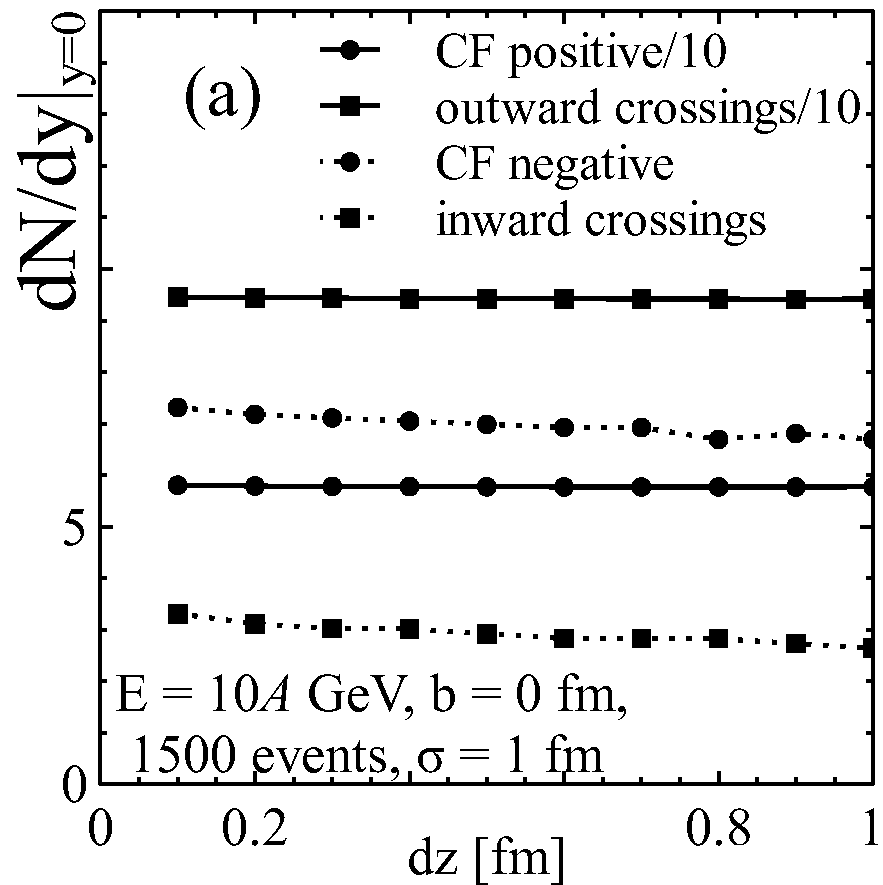
\includegraphics[height=4.6cm]{plots/cooper_frye/dz.pdf}
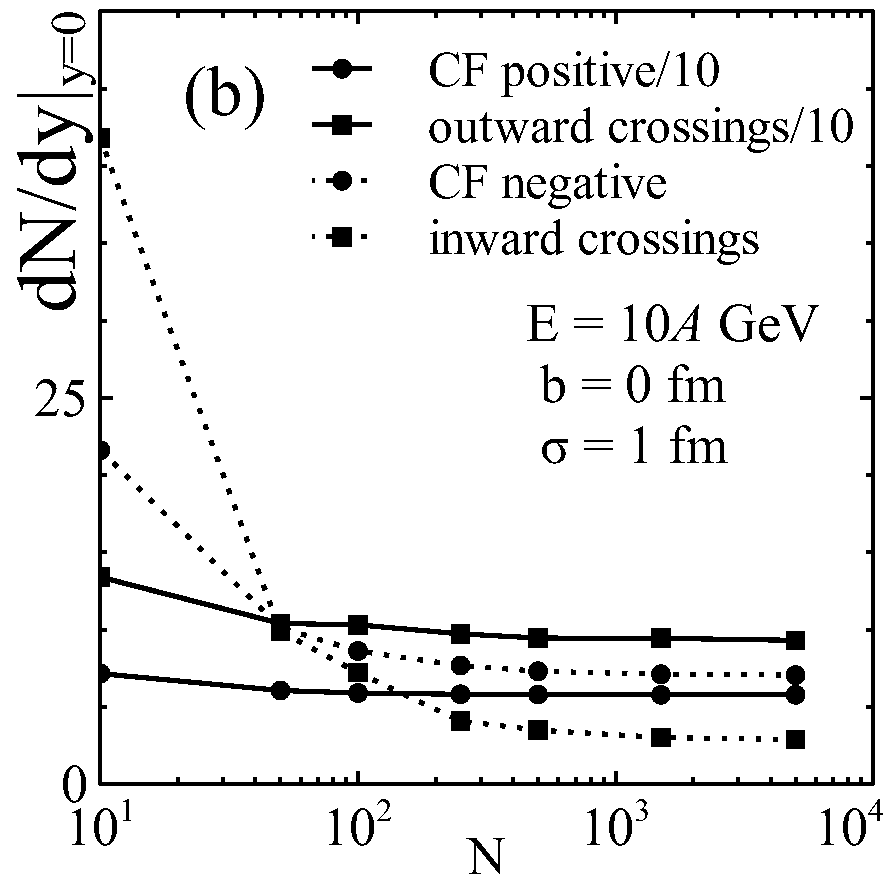
\includegraphics[height=4.6cm]{plots/cooper_frye/ev.pdf}
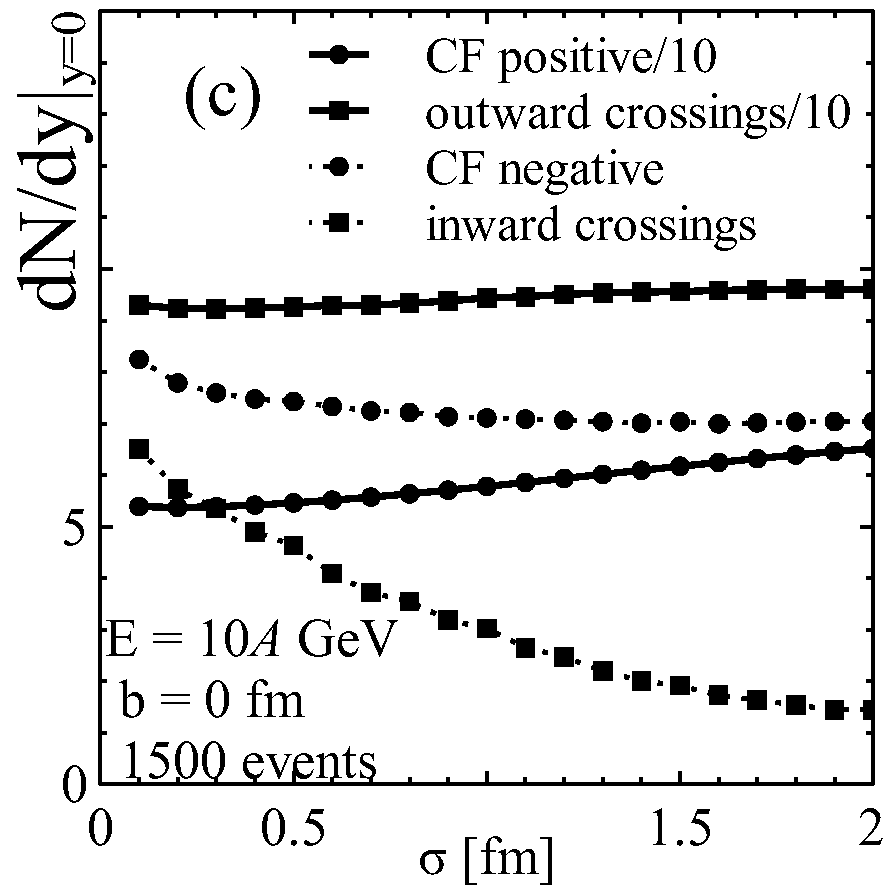
\includegraphics[height=4.6cm]{plots/cooper_frye/sig.pdf}
\caption{Sensitivity of results to internal parameters of the
  simulation: grid spacing along z axis, $dz$ (a), number of
  events, N (b) and the width $\sigma$ of Gaussian
  smearing (c). }
\label{Fig:Int_par}
\end{figure}

\begin{figure*}[htp]
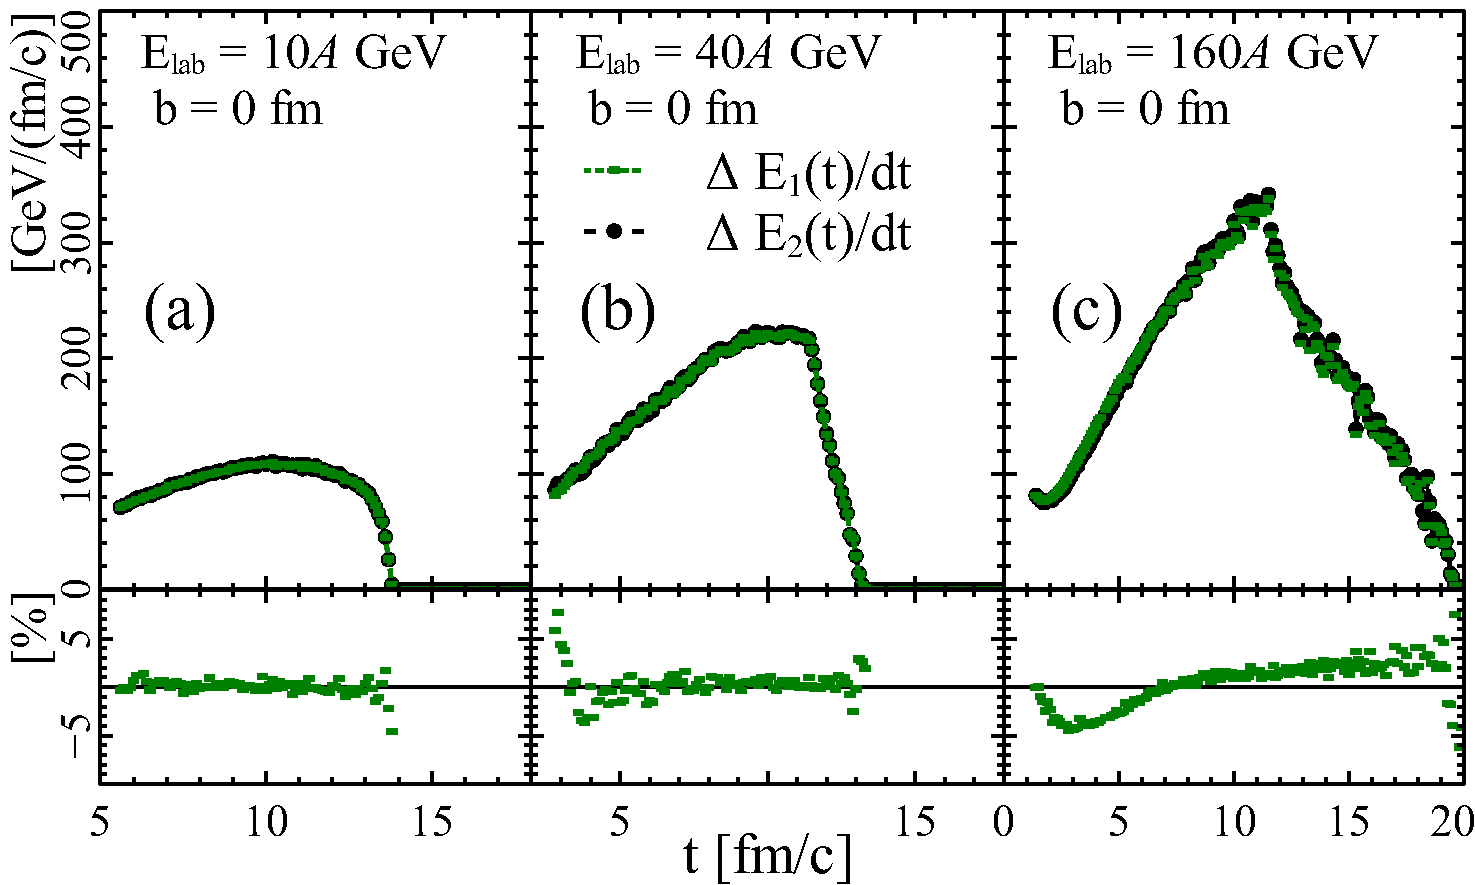
\includegraphics[height=7cm]{plots/cooper_frye/Econs.pdf}
\caption{ Energy flux through the surface at different
  times evaluated as actual flow,
  $\Delta E_1(t)/dt = \int_{t-dt}^{t} T^{\mu 0} d\sigma_{\mu}/dt$
  (circles), and as a difference in energy within the surface at
  different times, $\Delta E_2(t)/dt = (E_{in}(t) - E_{in}(t-dt))/dt$
  (rectangles). Lower panel shows the relative difference between
  these two measures in \%, and thus the conservation of energy in the
  calculation.}
\label{Fig:Econs}
\end{figure*}

Besides physical parameters like the beam energy, $\Elab$, and
centrality of the collision controlled by the impact parameter $b$,
our simulation contains internal parameters like grid spacing, the
width of the smearing Gaussian $\sigma$, and the number of events $N$.
Ideally, one should work in a region of internal parameters, where the
results are independent of them. To see how sensitive our results
are to these internal parameters, the positive and negative
contributions to the pion yield at midrapidity,
$\frac{dN}{dy}|_{y=0}$, at different values of these parameters are
evaluated.

The calculation is more sensitive to the grid spacing in z direction,
$dz$, than to the spacings in x and y directions, $dx$ and $dy$, since
gradients of $T^{\mu\nu}$ are largest in the longitudinal
direction. Although, as shown in Fig.~\ref{Fig:Int_par}~a), even the
sensitivity to $dz$ is weak over a reasonable range of values. The
main motivation for choosing the grid spacing and time step comes in
fact from the requirement of energy conservation discussed later.

The results are very sensitive to the small number of events (see
Fig.~\ref{Fig:Int_par}~b), but already $N = 500$ events provides
sufficient statistics for stable results.  To be on the safe side, we
have analyzed $N=1500$ events for our final results. Unfortunately,
our results are not completely independent of the width $\sigma$ of
the Gaussian smearing, as shown in Fig.~\ref{Fig:Int_par}~c). The
number of inward crossing UrQMD pions is most sensitive to
$\sigma$. Two effects play a role here: for small $\sigma$ the surface
still has large statistical fluctuations and small scale structures,
``lumps'' (See Fig.~2 of Ref~\cite{Huovinen:2002im}), whereas at large
$\sigma$ the smearing pushes transition surface further out in
space. Further out the densities are smaller, and the UrQMD particle
distributions are further away from equilibrium so that especially the
number of particles moving toward the center is strongly reduced.  We
choose $\sigma = 1$ fm as a reasonable value for our calculations, but
keep in mind that varying $\sigma$ in the range from 0.6 fm to 1.4 fm
causes $\sim$ 20 \% difference in the number of inward crossings. We
consider this a systematic error in our analysis, but fortunately this
uncertainty does not affect our main conclusions.

To check that energy is conserved in the coarse-graining procedure, we
evaluate the energy flow through the surface during the time step
$dt$, $\Delta E_1(t) = \int_{t-dt}^{t} T^{\mu 0} d\sigma_{\mu}$, and
compare it to the change in energy within the surface during the same
time step, $\Delta E_2(t) = E_{in}(t) - E_{in}(t-dt)$, where $E_{in}$
is total energy of particles inside the surface. Ideally
$\Delta E_1(t) = \Delta E_2(t)$ for any $dt$, but finite cell sizes
limit the precision and break the conservation of energy. The accuracy
of $\Delta E_1 \approx \Delta E_2$ improves when grid spacing and time
step are decreased. Fig.~\ref{Fig:Econs} shows the energy flux
through the surface and the relative difference between
$\Delta E_1(t)$ and $\Delta E_2(t)$ in central collisions at energies
$\Elab = 10$, 40, 160$A$ GeV. To achieve better than 5\% percent
accuracy at all times, small grid spacing is used with
$\Delta x = \Delta y = 1$ fm, $\Delta z$ = 0.3 fm, and time step
$\Delta t$ = 0.1 fm/c in collisions with $\Elab \le 80A$ GeV,
and an even finer grid with $\Delta x = \Delta y = 0.3$ fm, and
$\Delta z = 0.1$ fm for collisions at $\Elab = 160A$ GeV. When
integrated over the whole collision time, the violation of energy
conservation is less than 1\% at all collision energies. A similar check was performed
for the net baryon charge, and similar results were obtained.


\section{Magnitude of negative Cooper-Frye contributions estimated from the coarse-grained transport approach}
\label{sec:cf_Results}

\begin{figure}[htp]
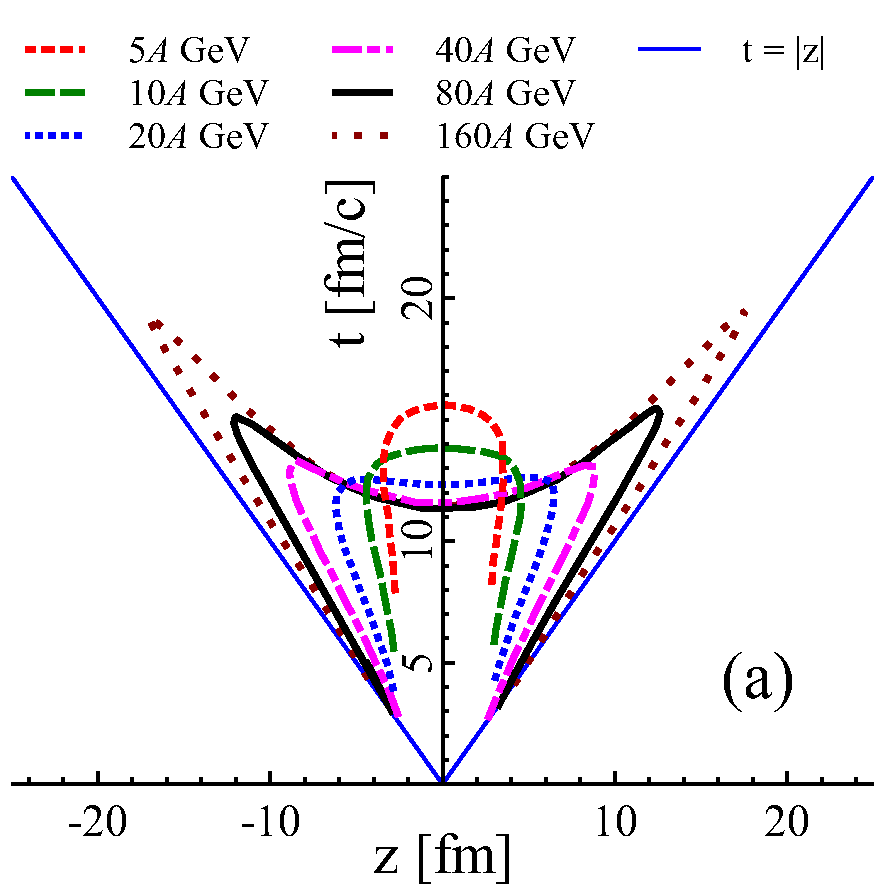
\includegraphics[height=6cm]{plots/cooper_frye/TZ.pdf}
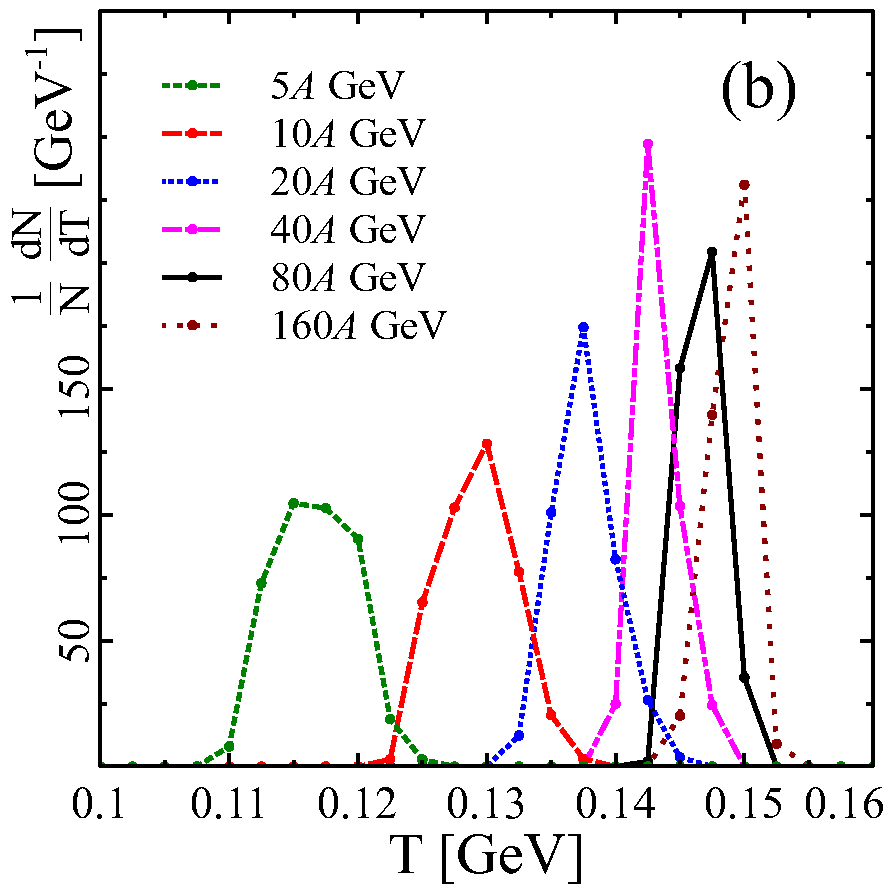
\includegraphics[height=6cm]{plots/cooper_frye/T_on_surf.pdf}
\caption{ Upper panel: Hypersurface of constant LRF
  energy density $\epsilon(t,0,0,z) = \epsilon_c = 0.3$
  GeV/fm$^3$. Lower panel: The fraction of hypersurface elements with
  (apparent) temperature $T$ in central Au+Au collisions at the
  collision energy of $\Elab = 5$, 10, 20, 40, 80, 160$A$ GeV.}
\label{Fig:surf}
\end{figure}

Let us start by investigating the properties of the transition
hypersurface itself as a function of beam energy. Figure
\ref{Fig:surf} depicts the surface $\Sigma$ in longitudinal direction
along the x axis. One can see that with increasing energy, the lifetime of
the system increases. This indicates longer lasting surface emission
(from space-like parts of the surface), which might lead to larger
negative contributions. On the other hand, with increasing energy the
longitudinal expansion leads to a larger volume of the final volume
emission (from time-like parts of the surface), which indicates
smaller negative contributions. Thus there are two competing effects,
and one has to carry out the actual calculation to find out how the
negative contributions depend on energy.

Distributions of the (apparent) temperature of the hypersurface
elements are shown on the right panel of Fig.~\ref{Fig:surf}. At each
collision energy the temperature distribution is rather narrow, which
means that the constant energy density surface approximately coincides
with a constant temperature surface. As well, the average temperature
increases with increasing collision energy as expected from thermal
model fits to particle yields~\cite{Andronic:2008gu}.

\begin{figure}[htp]
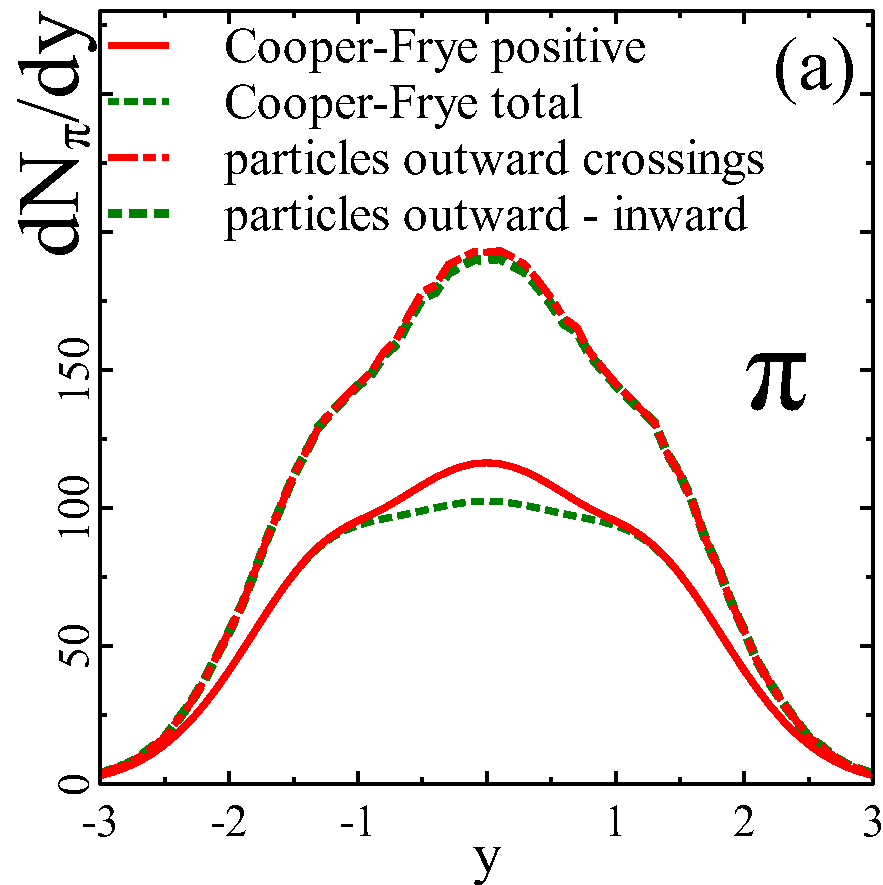
\includegraphics[width=5cm]{plots/cooper_frye/E40pi.pdf}
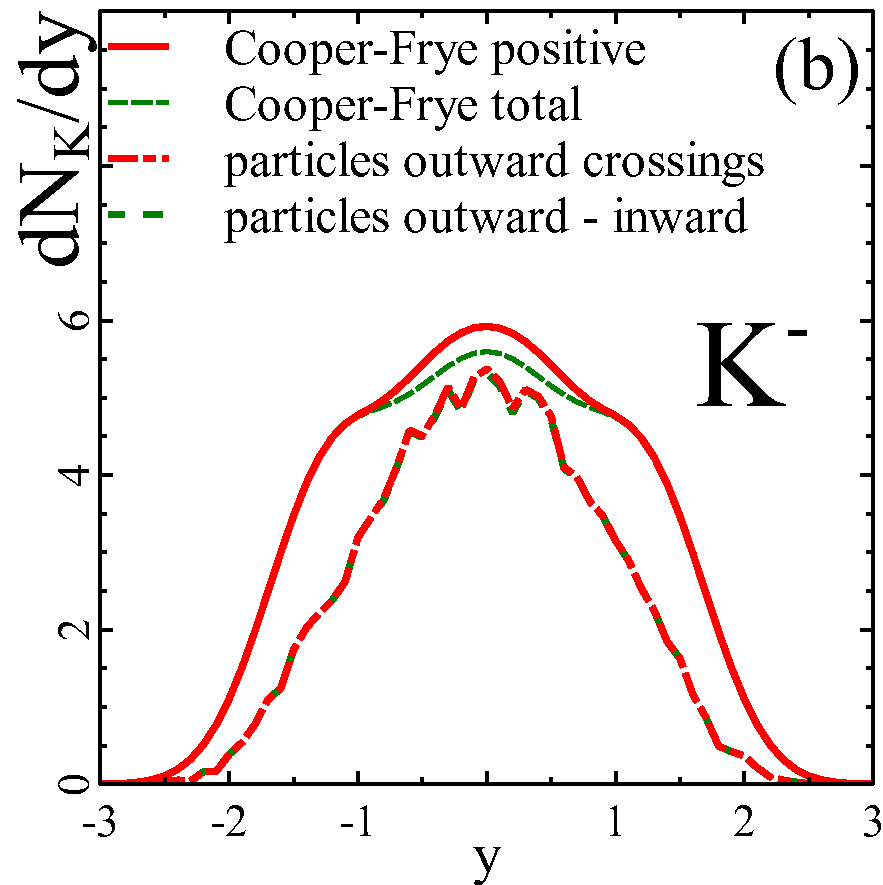
\includegraphics[width=5cm]{plots/cooper_frye/E40Kmi.pdf}
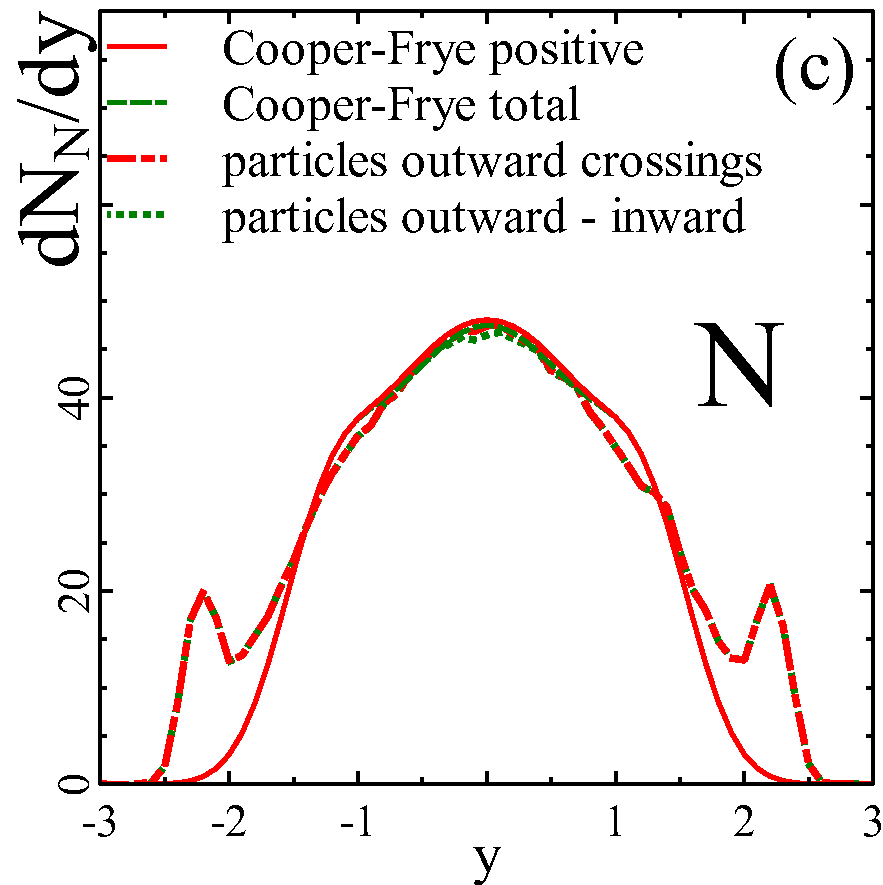
\includegraphics[width=5cm]{plots/cooper_frye/E40N.pdf}
\caption{ Rapidity distribution of identified particles
  obtained from Cooper-Frye formula on the surface $\Sigma$ and from
  explicit counting of particles that cross the same surface. Positive
  contributions and the net distribution, \emph{i.e.},
  positive-negative, are shown separately. 
  Central Au+Au collisions at $\Elab = 40$ \emph{A} GeV}
\label{Fig:spectra}
\end{figure}

Fig.~\ref{Fig:spectra} compares rapidity spectra of identified
particles in Au+Au collisions at $\Elab = 40$ \emph{A} GeV obtained by
Cooper-Frye calculation and by counting of the microscopic
particles. Even though, the results only for one
collision energy are shown, all results are qualitatively the same at all other
energies. If UrQMD is close to equilibrium on a surface at
$\epsilon_c = 0.3$ GeV/fm$^3$, both approaches should yield similar
distributions. At midrapidity this is the case for nucleons, and with
a lesser accuracy for kaons. $\Delta$'s, $\Lambda$'s, $\rho$'s and
$\eta$'s which are not shown in the figure depict a behavior similar
to nucleons. However, the pion yields are wildly different indicating
that pions are---and thus the entire system is---far away from
chemical equilibrium at least. To cancel the effect of
non-equilibrium and to visualize the differences in momentum distributions
we consider not the absolute value of the negative
contributions, but the ratio of negative to positive ones,
$(dN^-/dy)/(dN^+/dy)$ or $(dN^-/dp_T)/(dN^+/dp_T)$. From
Fig. \ref{Fig:spectra} it is also apparent that the magnitude of the
negative contributions is always small compared to the positive ones
as expected.


\begin{figure}[htp]
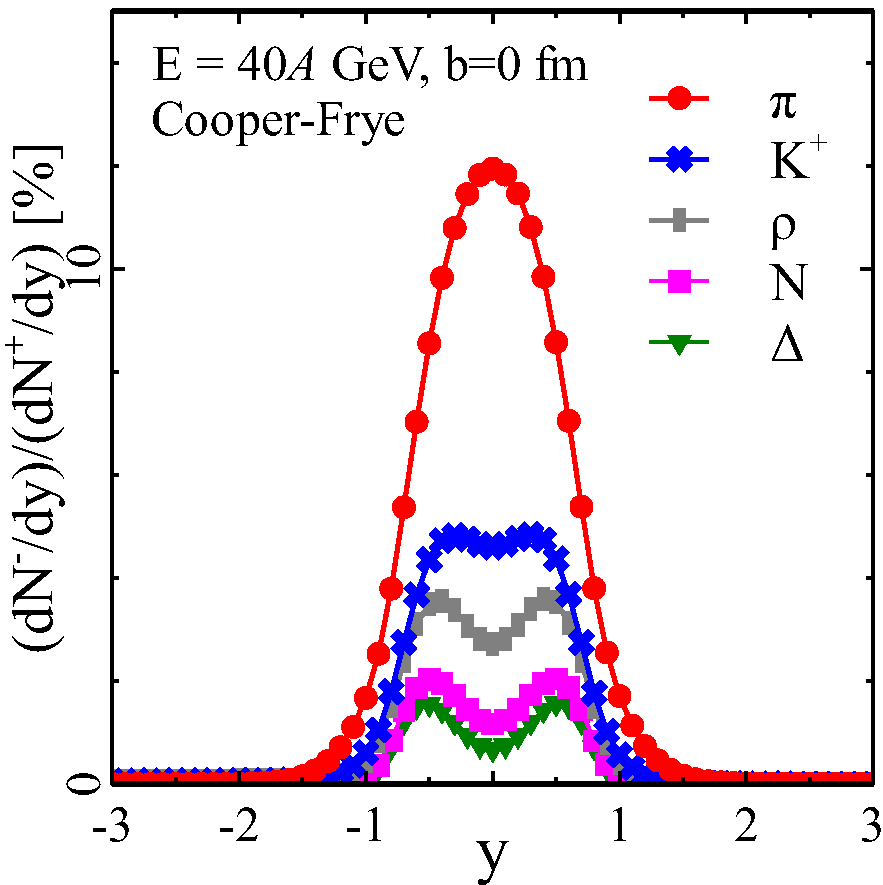
\includegraphics[width=7cm]{plots/cooper_frye/neg_contr_mass.pdf}
\caption{ Rapidity distribution of the ratio of negative
  to positive contributions for different hadron species: pions
  (circles), $K^{+}$ (crosses), $\rho$ (bars), nucleons (rectangles),
  and deltas (triangles).  Cooper-Frye calculation in central Au+Au
  collisions at $\Elab = 40A$ GeV.}
\label{Fig:neg_contr_pmass}
\end{figure}

The dependence of the ratio $(dN^-/dy)/(dN^+/dy)$ on the hadron type
is illustrated in Fig.~\ref{Fig:neg_contr_pmass} by the Cooper-Frye
results. Since for all cases, the microscopic negative contributions
of backstreaming particles are much smaller than the Cooper-Frye ones
we concentrate on showing the maximal effect. Surface temperature and
velocity profiles are identical for all hadrons, so the plot
demonstrates first of all the effect of particle mass. One can see
that the average value of $(dN^-/dy)/(dN^+/dy)$ decreases with
particle mass. This can be understood by considering a small volume of
fluid in its rest frame, and a space-like surface moving through it
with a velocity $0<v_{surf}<c$ so that lower density, \emph{i.e.},
outside, is in the negative direction. To be counted as a negative
contribution, a particle must enter the fluid, and thus have a larger
velocity than the surface. Average thermal velocity decreases with
increasing mass, and therefore the heavier the particle, the fewer of
them cross the surface inward. Since relative negative contributions
for pions are several times larger than for other hadrons,
in the following only pions will be considered.


\begin{figure}[htp]
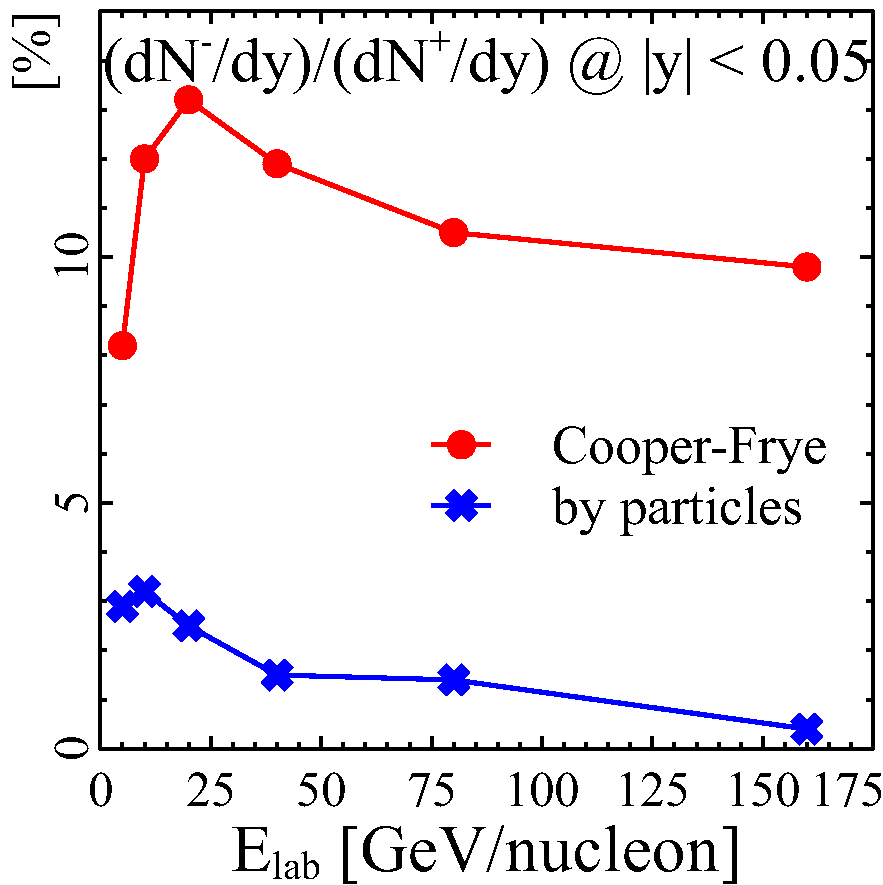
\includegraphics[width=7cm]{plots/cooper_frye/neg_vs_E.pdf}
\caption{ The ratio of negative to positive
  contributions on the $\epsilon(t,x,y,z) = \epsilon_c = 0.3$
  GeV/fm$^3$ surface for pions at midrapidity in central Au+Au
  collisions at various collision energies. Circles depict Cooper-Frye
  result and rectangles the explicit counting of UrQMD particles.}
\label{Fig:neg_contr_Ecoll}
\end{figure}

As could be seen in Fig.~\ref{Fig:spectra}, imposing equilibrium for
Cooper-Frye calculation leads to significantly larger negative to
positive contribution ratio at midrapidity than the counting of UrQMD
particles. As shown in Fig.~\ref{Fig:neg_contr_Ecoll} this holds for
all the considered energies, showing that the system is out of
not only chemical, but also of kinetic equilibrium. Either the
collective flow velocity of pions is different from the collective
velocity of other particles \cite{Sorge:1995pw,Pratt:1998gt} or the
dissipative corrections to pion distribution are very large. It was
also checked that the relative microscopic negative contributions are
much smaller in UrQMD at all centralities, for all particle species,
and on isosurfaces of energy density $\epsilon_c = 0.3$ and 0.6
GeV/fm$^3$.

On the other hand, the trend as a function of collision energy in
Cooper-Frye and UrQMD calculations is the same: both curves have a
maximum at 10-20$A$ GeV and then decrease with increasing energy. This
behavior is a result of a complicated interplay of several factors:
temperature, relative velocities between surface and fluid, and
relative amounts of volume and surface emission, \emph{i.e.}, emission
from the time- and space-like parts of the surface. To gain some
insight all these factors are considered separately. The same argument
used to explain the sensitivity of negative contributions to particle
mass, explains why larger temperature leads to larger negative
contributions. Temperature on the constant density surface grows with
increasing collision energy (see Fig.~\ref{Fig:surf}), which would
lead one to expect an increase of negative contributions with
increasing collision energy. On the other hand, larger relative
velocity between the fluid and surface reduces the negative
contributions (again the same argument), and one can see that the average
relative velocity increases with increasing collision energy. Finally,
as argued when discussing Fig.~\ref{Fig:surf}, the
larger the collision energy, the larger the fraction of volume
emission. Which, as mentioned, reduces the negative contributions.

\begin{figure}[htp]
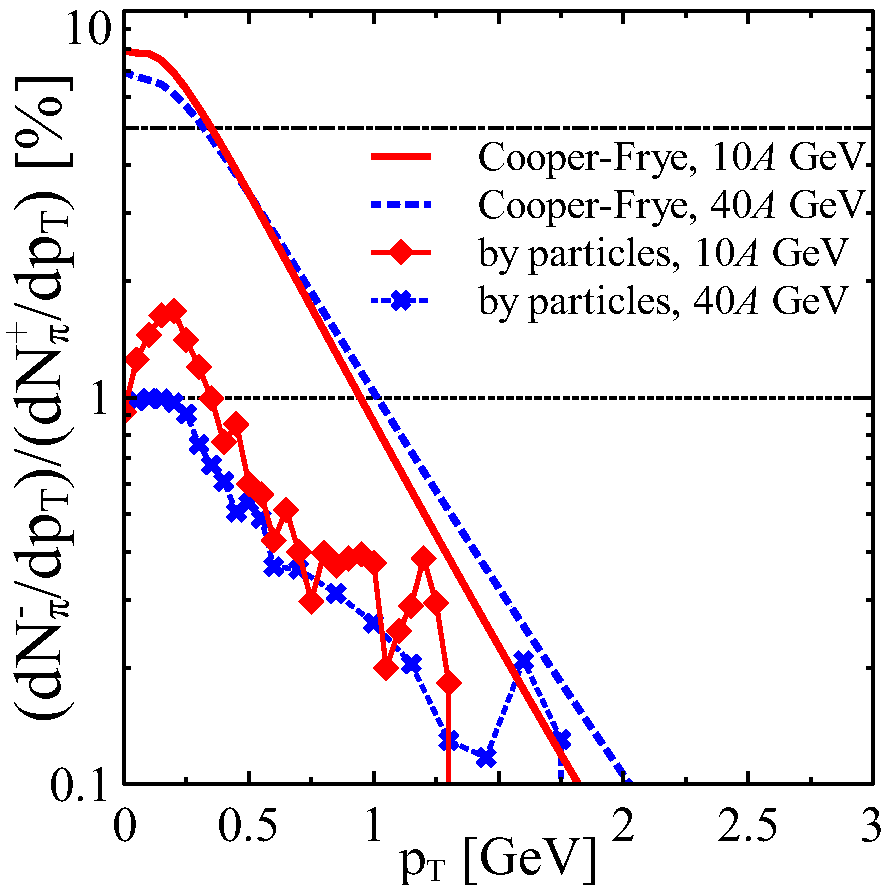
\includegraphics[width=7cm]{plots/cooper_frye/pt_binned_negcontr_pi_E40rebinned.pdf}
\caption{ The ratio of negative to positive pion
  contributions as a function of transverse momentum at midrapidity in
  central Au+Au collisions at $\Elab = 5$, 10, 20, 40, 80$A$ GeV.}
\label{Fig:neg_contr_pt}
\end{figure}

It is instructive to evaluate the negative contributions as function
of transverse momentum $p_T$ as well, as shown in
Fig.~\ref{Fig:neg_contr_pt} for Cooper-Frye calculation and "by
particles". One can see that the largest negative contributions are
located at small $p_T$, which means that one can reduce the
uncertainty caused by the negative contributions by a low $p_T$
cut. Also as a function of transverse momentum, the amount of
microscopically backward streaming particles is much smaller than in
an equilibrium scenario.

When discussing Fig.~\ref{Fig:neg_contr_Ecoll} it was mentioned that,
independent of the energy density of the surface, the negative
contributions are much smaller when counting the UrQMD
particles. Furthermore, in Cooper-Frye calculations the strength of
the negative contributions depends on the value of $\epsilon_c$ where
the distributions are evaluated as shown in
Fig.~\ref{Fig:neg_contr_e0}. Larger $\epsilon_c$ leads to larger
negative contribution at midrapidity and lower at back- and forward
rapidities. This result arises from interplay of two factors: larger
temperature and smaller average $v_{rel}$ for larger energy
density. Quite surprisingly the negative contributions evaluated by
counting the UrQMD particles is almost independent of the value of
$\epsilon_c$. This indicates that even in much higher temperature
$T\sim 155$--160 MeV the microscopic system is not fully thermalised.

\begin{figure}[htp]
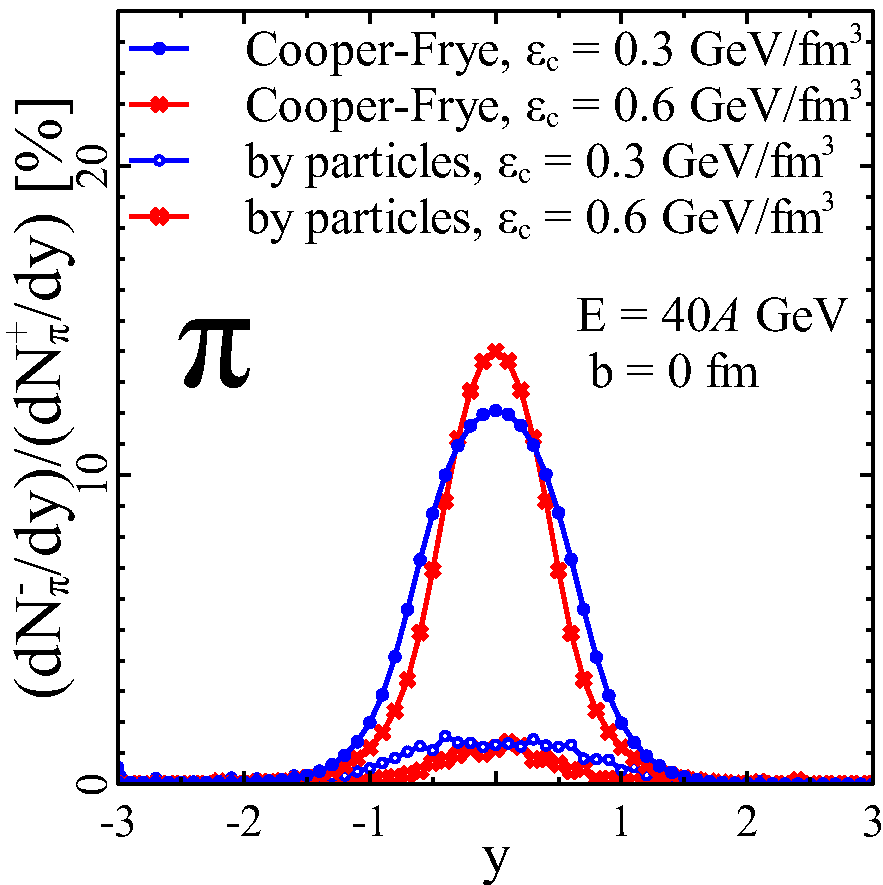
\includegraphics[width=7cm]{plots/cooper_frye/piym_new.pdf}
\caption{ Rapidity distribution of the ratio of negative
  to positive contributions for pions on
  $\epsilon(t,x,y,z) = \epsilon_c = 0.3$ GeV/fm$^3$ (circles) and
  $\epsilon_c = 0.6$ GeV/fm$^3$ (crosses) surfaces in central Au+Au
  collisions at $\Elab = 40\ A$ GeV. Full symbols correspond to
  Cooper-Frye calculation and open symbols to explicit counting of
  UrQMD particles.}
\label{Fig:neg_contr_e0}
\end{figure}

The dependence of the contribution ratio on centrality is shown in
Fig.~\ref{Fig:neg_contr_b}. The negative contributions decrease with
decreasing centrality because the more peripheral the collision, the
larger the fraction of time-like hypersurface elements. This behavior
is illustrated in the right panel of Fig.~\ref{Fig:neg_contr_b}. In
the limit of very peripheral collisions the lifetime of the system
becomes zero, and thus the surface is time-like everywhere and there
are no negative contributions at all. Temperature and relative
velocities appear to be less important factors in this case than the
relative amount of time-like and space-like hypersurface elements.

\begin{figure}[htp]
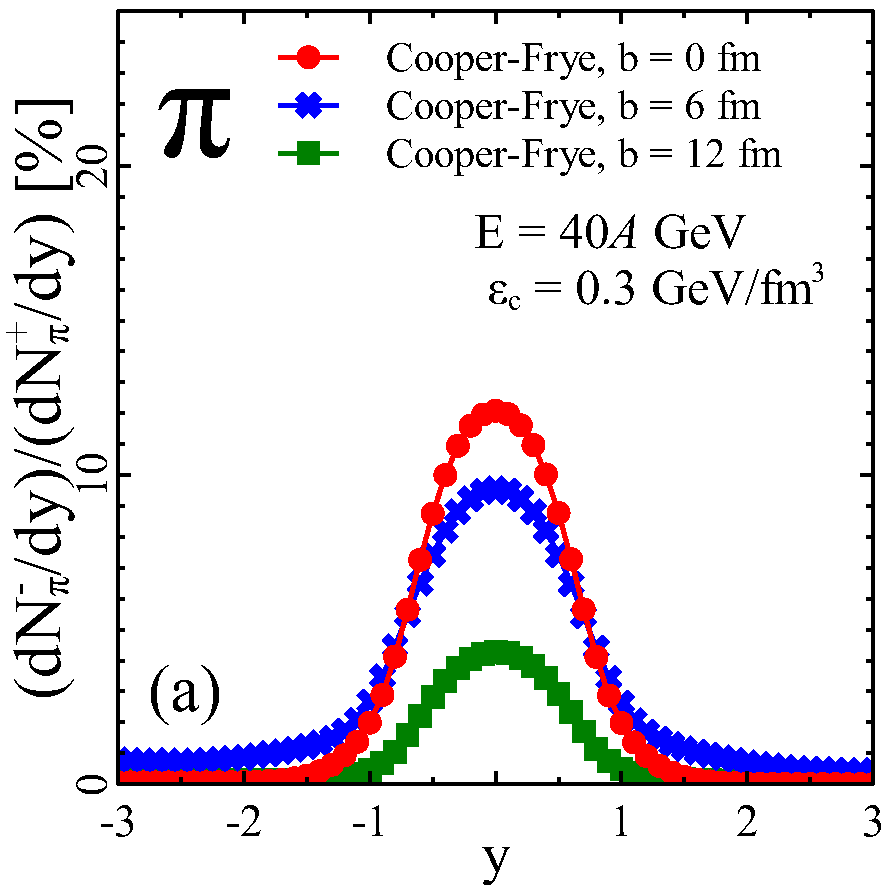
\includegraphics[height=7cm]{plots/cooper_frye/neg_contr_b_v2.pdf}
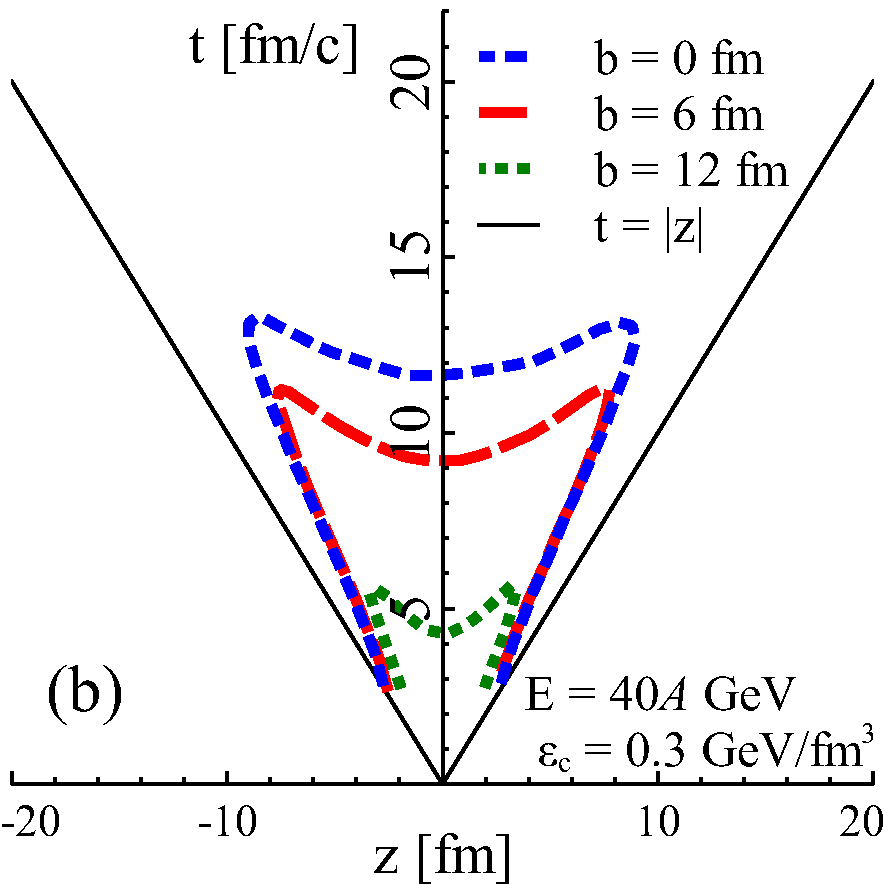
\includegraphics[height=7cm]{plots/cooper_frye/TZ_vs_b.pdf}
\caption{ Upper panel: Rapidity distribution of the
  ratio of negative to positive contributions for pions in Au+Au
  collisions at $\Elab = 40\ A$ GeV at various centralities: $b=0$
  (circles), $b = 6$ fm (crosses) and $b = 12$ fm (rectangles). Lower
  panel: hypersurfaces along the z axis in the same collisions at the
  same centralities.}
\label{Fig:neg_contr_b}
\end{figure}

Let us finally compare our results to previous studies. In
\cite{Huovinen:2012is} negative contributions were evaluated on the
$\epsilon = 0.3$ GeV/fm$^3$ transition surface of a hybrid model at
SPS and RHIC energies---$\Elab = 160A$ GeV and
$\sqrt{s_\mathrm{NN}} = 200$ GeV, respectively---and found to be
around $(dN^{-}_{\pi}/dy)/(dN^{+}_{\pi}/dy) \simeq$ 13\% and 9\% at
$y=0$. The negative contributions for 160$A$ GeV are slightly larger
than in our calculation. The reason for this discrepancy lies in the
difference of the velocity profiles on the hypersurfaces: In
hydrodynamics the average relative velocity between flow and surface
is smaller than in our transport-based approach, which leads to larger
negative contributions.

\section{Summary and discussion}

The assumptions of hybrid and hydrodynamical approaches at the end of the
hydrodynamical evolution lead to the appearance of Cooper-Frye negative
contributions - negative numbers of particles produced by the Cooper-Frye
formula at particlization on the hypersurface elements with a space-like
normal. At high collision energies at midrapidity --- the kinematic region probed by
RHIC and LHC --- the Cooper-Frye negative contributions are negligible. However,
at intermediate energies they were not studied before.

Here negative Cooper-Frye contributions and
backscattering were investigated using a coarse-grained transport
approach. Au+Au collisions at $\Elab = 5$--$160\ A$ GeV energies have
been simulated with UrQMD, and a hypersurface $\Sigma$ of constant
Landau rest frame energy density has been constructed. On this surface
two quantities were computed: The ratio of Cooper-Frye negative
to positive contributions, which assumes local thermal equilibrium,
and the ratio of UrQMD particles crossing $\Sigma$ inward to crossing
$\Sigma$ outward, which assumes no equilibrium.

It was found that at all collision energies the ratio of inward to outward
moving particles calculated counting the UrQMD particles is much
smaller than the same ratio calculated assuming equilibrium,
\emph{i.e.}, the Cooper-Frye negative to positive ratio. This finding
poses a question to the construction of hybrid models, and the
treatment of freeze-out in hydrodynamical models: If the cascade leads
to distributions nowhere near equilibrium, how are the hydrodynamical
and cascade stages to be connected in a consistent fashion? On the
other hand, this result shows that an ideal fluid dynamics hybrid
approach contains the worst case scenario for negative contributions
and even then they are on the order of max.~$15\%$ for the pion yield
at midrapidity. What remains to be seen, however, is whether one could
get closer to the UrQMD result with dissipative corrections
to the distribution function of Cooper-Frye, or whether the deviations
from equilibrium are so large that dissipative expansion is not
feasible.

The largest observed impact of negative contributions is to pion
rapidity spectrum at midrapidity in central collisions. In thermally
equilibrated Cooper-Frye calculations it constitutes 8--13\%, but only
0.5--4\% in the counting of UrQMD particles. The Cooper-Frye value
roughly agrees with the values obtained previously for hydrodynamics
at 160 GeV. Several systematic features were found in these ratios. They
are smaller for larger hadron mass and therefore largest for
pions. The relative negative contributions decrease as a function of
collision energy and by going from central to peripheral
collisions. On the other hand, they increase if a higher energy
density is chosen as a surface criterion. The small scale structures
on the surface, its ``lumpiness'', play a significant role: If the
surface is not smooth enough both ratios can increase
dramatically. Therefore, an interesting future study could be to
compare single fluctuating events to the averaged result.
